% !TEX root = ../master-thesis.tex

% tweezer_movement.tex

% \subsection{Tweezer movement} \label{subsec:tweezer-movement}




% \textbf{Tweezer movement}.
In experiments aiming at deterministic preparation and site-resolved imaging of individual ultracold atoms, precise and robust control over tweezer positions is crucial. In the present setup, while the Matter-Wave Magnifier (MWM) remains under development, single-atom imaging is achieved by initially positioning optical tweezers sufficiently far apart to individually resolve atoms. Specifically, atoms are loaded from the optical dipole trap (ODT) into tweezer potentials at an initial separation of $5\mu$m. Subsequently, this spacing is gradually increased to approximately $50\mu$m by smoothly varying the driving frequencies of the acousto-optic deflectors (AODs), enabling direct optical resolution without additional magnification.

% \textbf{Transport trajectory optimization.}
The protocol chosen for tweezer translation critically influences the fidelity of atom transport. Naively, atoms can be moved by linearly ramping tweezer frequencies; however, such linear trajectories often lead to significant atom loss due to non-adiabatic excitations induced by abrupt changes in acceleration. To mitigate these losses, a smoother trajectory known as the Minimum-Jerk Trajectory (MJT) is employed. This trajectory is derived by minimizing the functional associated with the time-integrated square of the third derivative of the position, known as the jerk $j(t) = \dddot{x}(t)$:
\begin{equation}
\mathcal{J}[x(t)] = \int_{0}^{T} \left(\frac{d^3 x(t)}{dt^3}\right)^2 dt,
\label{eq:mjt-functional}
\end{equation}
where $x(t)$ denotes the position and $T$ the total transport duration. Minimization of Eq.~\eqref{eq:mjt-functional}, subject to the boundary conditions of initial and final positions $x(0) = x_i$, $x(T) = x_f$, and zero initial and final velocities and accelerations, yields a polynomial form:
\begin{equation}
x(t) = x_i + (x_f - x_i)\left[10\left(\frac{t}{T}\right)^3 - 15\left(\frac{t}{T}\right)^4 + 6\left(\frac{t}{T}\right)^5\right].
\label{eq:mjt-solution}
\end{equation}
This smooth polynomial interpolation minimizes abrupt changes in acceleration, thereby reducing non-adiabatic excitation and atom loss during transport.

\begin{figure}
\centering
\addletter{85}{a}
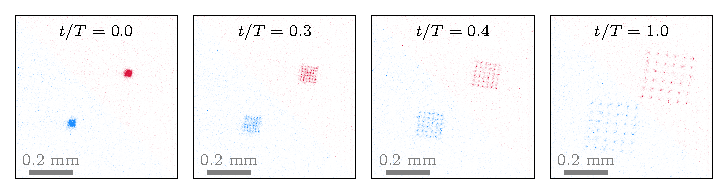
\includegraphics{fig-py/movement-inset.pdf} \\
\addletter{115}{b}
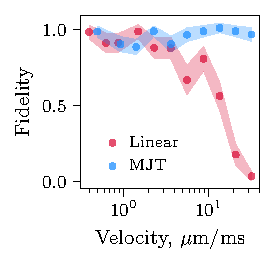
\includegraphics{fig-py/movement-1.pdf}
\hspace{1cm}
\addletter{115}{c}
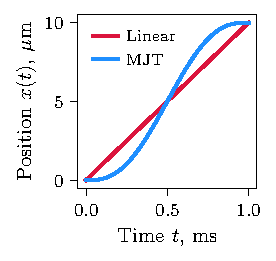
\includegraphics{fig-py/movement-2.pdf}
\caption{
\textbf{Characterization of tweezer transport protocols.}
(a) Snapshots at different fractions of the total transport duration, illustrating atom movement between initial and target tweezer positions during a typical experimental run.
(b) Comparison of transport fidelity as a function of velocity for the Minimum-Jerk Trajectory (MJT) and linear trajectory. Fidelity is defined as the probability of detecting an atom after transport, conditional on its initial presence.
(c) Position versus time curves for MJT and linear transport trajectories.
Data points correspond to measurements, shaded areas represent standard deviation across realizations.
}
\label{fig:movement}
\end{figure}


% \textbf{Experimental characterization of trajectories.}
To experimentally validate the efficacy of MJT compared to linear transport, systematic measurements were conducted. The fidelity of transport is defined as the probability of detecting an atom after transport, conditional upon its initial presence. As depicted in Fig.~\ref{fig:movement}b, the MJT significantly outperforms the linear trajectory across a broad range of transport velocities. These measurements are obtained by initially holding atoms stationary for a fixed duration, thereby establishing a baseline population expected without transport-induced losses. Subsequently, atoms are transported along a zigzag path (forward and backward), and transport fidelity is measured relative to this baseline. Given the relatively low mass of $^6$Li atoms, high transport velocities are achievable. Indeed, at typical experimental transport velocities of approximately $10\mu$m/ms, MJT achieves fidelities exceeding 99\%, as demonstrated in Fig.~\ref{fig:movement}b. This highlights MJT as the trajectory of choice for efficient and robust tweezer movement.

% \textbf{Trajectory profiles and experimental snapshots.}
Detailed position versus time curves for both linear and MJT trajectories are shown in Fig.\ref{fig:movement}c. The MJT profile distinctly smooths acceleration and deceleration phases compared to the linear ramp, clearly illustrating the reduction in jerk. Correspondingly, experimental snapshots at various fractions of the total transport duration, depicted in Fig.\ref{fig:movement}a, visually confirm smooth and uniform atomic redistribution between initial and final positions. Each snapshot represents fluorescence images averaged over ten experimental realizations, confirming reproducible atom transport without significant losses or heating.

In summary, the implementation and systematic characterization of MJT for tweezer translation provides a critical improvement in transport fidelity compared to simple linear movements. The derived and experimentally validated MJT ensures minimal atom loss, thereby facilitating precise atom arrangement. 

